% Options for packages loaded elsewhere
\PassOptionsToPackage{unicode}{hyperref}
\PassOptionsToPackage{hyphens}{url}
\PassOptionsToPackage{dvipsnames,svgnames,x11names}{xcolor}
%
\documentclass[
  letterpaper,
  DIV=11,
  numbers=noendperiod]{scrartcl}

\usepackage{amsmath,amssymb}
\usepackage{lmodern}
\usepackage{iftex}
\ifPDFTeX
  \usepackage[T1]{fontenc}
  \usepackage[utf8]{inputenc}
  \usepackage{textcomp} % provide euro and other symbols
\else % if luatex or xetex
  \usepackage{unicode-math}
  \defaultfontfeatures{Scale=MatchLowercase}
  \defaultfontfeatures[\rmfamily]{Ligatures=TeX,Scale=1}
\fi
% Use upquote if available, for straight quotes in verbatim environments
\IfFileExists{upquote.sty}{\usepackage{upquote}}{}
\IfFileExists{microtype.sty}{% use microtype if available
  \usepackage[]{microtype}
  \UseMicrotypeSet[protrusion]{basicmath} % disable protrusion for tt fonts
}{}
\makeatletter
\@ifundefined{KOMAClassName}{% if non-KOMA class
  \IfFileExists{parskip.sty}{%
    \usepackage{parskip}
  }{% else
    \setlength{\parindent}{0pt}
    \setlength{\parskip}{6pt plus 2pt minus 1pt}}
}{% if KOMA class
  \KOMAoptions{parskip=half}}
\makeatother
\usepackage{xcolor}
\setlength{\emergencystretch}{3em} % prevent overfull lines
\setcounter{secnumdepth}{-\maxdimen} % remove section numbering
% Make \paragraph and \subparagraph free-standing
\ifx\paragraph\undefined\else
  \let\oldparagraph\paragraph
  \renewcommand{\paragraph}[1]{\oldparagraph{#1}\mbox{}}
\fi
\ifx\subparagraph\undefined\else
  \let\oldsubparagraph\subparagraph
  \renewcommand{\subparagraph}[1]{\oldsubparagraph{#1}\mbox{}}
\fi


\providecommand{\tightlist}{%
  \setlength{\itemsep}{0pt}\setlength{\parskip}{0pt}}\usepackage{longtable,booktabs,array}
\usepackage{calc} % for calculating minipage widths
% Correct order of tables after \paragraph or \subparagraph
\usepackage{etoolbox}
\makeatletter
\patchcmd\longtable{\par}{\if@noskipsec\mbox{}\fi\par}{}{}
\makeatother
% Allow footnotes in longtable head/foot
\IfFileExists{footnotehyper.sty}{\usepackage{footnotehyper}}{\usepackage{footnote}}
\makesavenoteenv{longtable}
\usepackage{graphicx}
\makeatletter
\def\maxwidth{\ifdim\Gin@nat@width>\linewidth\linewidth\else\Gin@nat@width\fi}
\def\maxheight{\ifdim\Gin@nat@height>\textheight\textheight\else\Gin@nat@height\fi}
\makeatother
% Scale images if necessary, so that they will not overflow the page
% margins by default, and it is still possible to overwrite the defaults
% using explicit options in \includegraphics[width, height, ...]{}
\setkeys{Gin}{width=\maxwidth,height=\maxheight,keepaspectratio}
% Set default figure placement to htbp
\makeatletter
\def\fps@figure{htbp}
\makeatother

\KOMAoption{captions}{tableheading}
\makeatletter
\makeatother
\makeatletter
\makeatother
\makeatletter
\@ifpackageloaded{caption}{}{\usepackage{caption}}
\AtBeginDocument{%
\ifdefined\contentsname
  \renewcommand*\contentsname{Table of contents}
\else
  \newcommand\contentsname{Table of contents}
\fi
\ifdefined\listfigurename
  \renewcommand*\listfigurename{List of Figures}
\else
  \newcommand\listfigurename{List of Figures}
\fi
\ifdefined\listtablename
  \renewcommand*\listtablename{List of Tables}
\else
  \newcommand\listtablename{List of Tables}
\fi
\ifdefined\figurename
  \renewcommand*\figurename{Figure}
\else
  \newcommand\figurename{Figure}
\fi
\ifdefined\tablename
  \renewcommand*\tablename{Table}
\else
  \newcommand\tablename{Table}
\fi
}
\@ifpackageloaded{float}{}{\usepackage{float}}
\floatstyle{ruled}
\@ifundefined{c@chapter}{\newfloat{codelisting}{h}{lop}}{\newfloat{codelisting}{h}{lop}[chapter]}
\floatname{codelisting}{Listing}
\newcommand*\listoflistings{\listof{codelisting}{List of Listings}}
\makeatother
\makeatletter
\@ifpackageloaded{caption}{}{\usepackage{caption}}
\@ifpackageloaded{subcaption}{}{\usepackage{subcaption}}
\makeatother
\makeatletter
\@ifpackageloaded{tcolorbox}{}{\usepackage[many]{tcolorbox}}
\makeatother
\makeatletter
\@ifundefined{shadecolor}{\definecolor{shadecolor}{rgb}{.97, .97, .97}}
\makeatother
\makeatletter
\makeatother
\ifLuaTeX
  \usepackage{selnolig}  % disable illegal ligatures
\fi
\IfFileExists{bookmark.sty}{\usepackage{bookmark}}{\usepackage{hyperref}}
\IfFileExists{xurl.sty}{\usepackage{xurl}}{} % add URL line breaks if available
\urlstyle{same} % disable monospaced font for URLs
\hypersetup{
  pdftitle={Data Analytics Workshop},
  pdfauthor={Business Data Laboratory},
  colorlinks=true,
  linkcolor={blue},
  filecolor={Maroon},
  citecolor={Blue},
  urlcolor={Blue},
  pdfcreator={LaTeX via pandoc}}

\title{Data Analytics Workshop}
\author{Business Data Laboratory}
\date{}

\begin{document}
\maketitle
\ifdefined\Shaded\renewenvironment{Shaded}{\begin{tcolorbox}[borderline west={3pt}{0pt}{shadecolor}, boxrule=0pt, enhanced, interior hidden, sharp corners, breakable, frame hidden]}{\end{tcolorbox}}\fi

\hypertarget{agenda}{%
\subsection{Agenda}\label{agenda}}

\begin{itemize}
\item
  Intro {👋}
\item
  Today's Take-away {📋}
\item
  Q/A
\item
  Thank you
\end{itemize}

\hypertarget{todays-take-away}{%
\subsection{Today's Take-away}\label{todays-take-away}}

\begin{enumerate}
\def\labelenumi{\arabic{enumi}.}
\tightlist
\item
  Why a Career as a Data Analyst?
\item
  Why now?
\item
  Why learn from Us?
\item
  Our Instructors
\item
  Time for today's Workshop
\end{enumerate}

\hypertarget{why-a-career-as-a-data-analyst}{%
\section{Why a Career as a Data
Analyst?}\label{why-a-career-as-a-data-analyst}}

1 {2 3 4 5 6}

\begin{center}\rule{0.5\linewidth}{0.5pt}\end{center}

\hypertarget{what-does-a-data-analyst-do}{%
\subsection{What does a Data Analyst
do?}\label{what-does-a-data-analyst-do}}

1 {2 3 4 5 6}

\begin{itemize}
\tightlist
\item
  Source and gather data,
\item
  Clean and organize it
\item
  Use data to reach meaningful conclusions
\item
  Communicate results through visuals and reports
\end{itemize}

\begin{center}\rule{0.5\linewidth}{0.5pt}\end{center}

\hypertarget{why-a-career-now-as-a-data-analyst}{%
\subsection{Why a career now, as a data
analyst?}\label{why-a-career-now-as-a-data-analyst}}

1 {2 3 4 5 6}

\begin{itemize}
\tightlist
\item
  Salaries range from 168,000 NGN to 481,000 NGN or more for experienced
  Data Analysts
\item
  Remote/Hybrid work option
\item
  Freelancing
\item
  Start your own consulting
\end{itemize}

\hypertarget{why-learn-from-business-data-laboratory}{%
\section{Why learn from Business Data
Laboratory?}\label{why-learn-from-business-data-laboratory}}

{1} 2 {3 4 5 6}

\begin{center}\rule{0.5\linewidth}{0.5pt}\end{center}

\hypertarget{our-classes---in-person}{%
\subsection{Our Classes - In-person}\label{our-classes---in-person}}

{1} 2 {3 4 5 6}

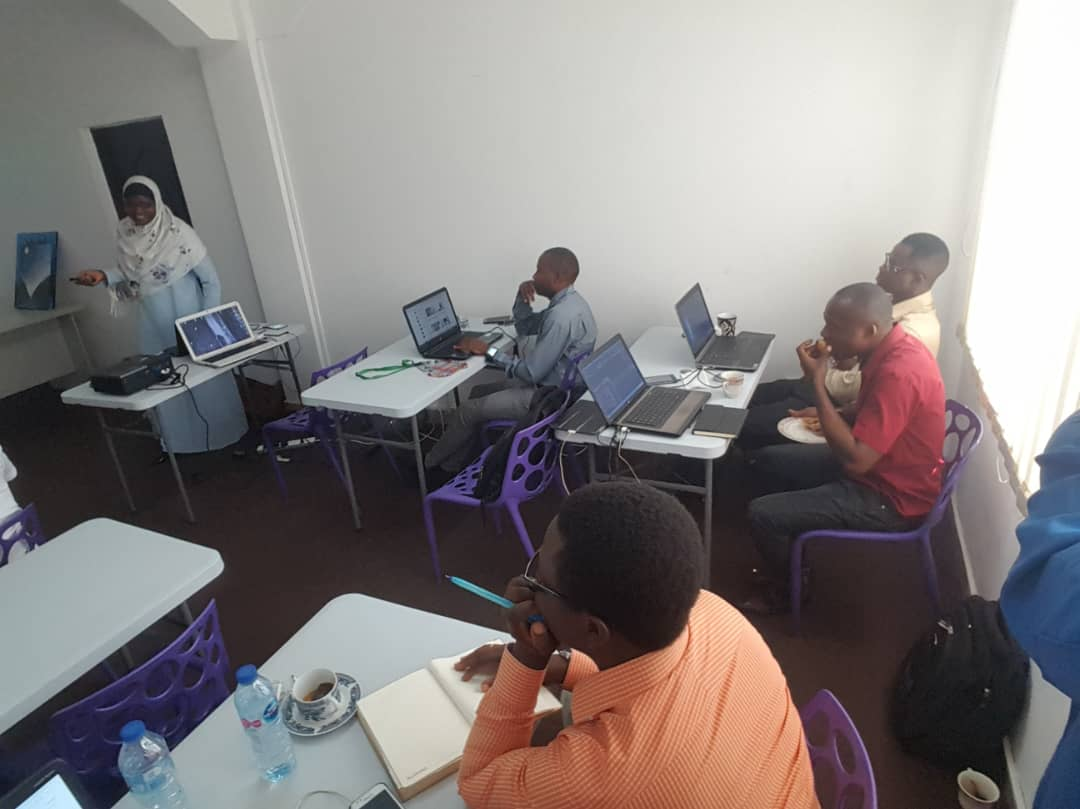
\includegraphics[width=5.19792in,height=5.97917in]{images/trainings/pics1.jpeg}

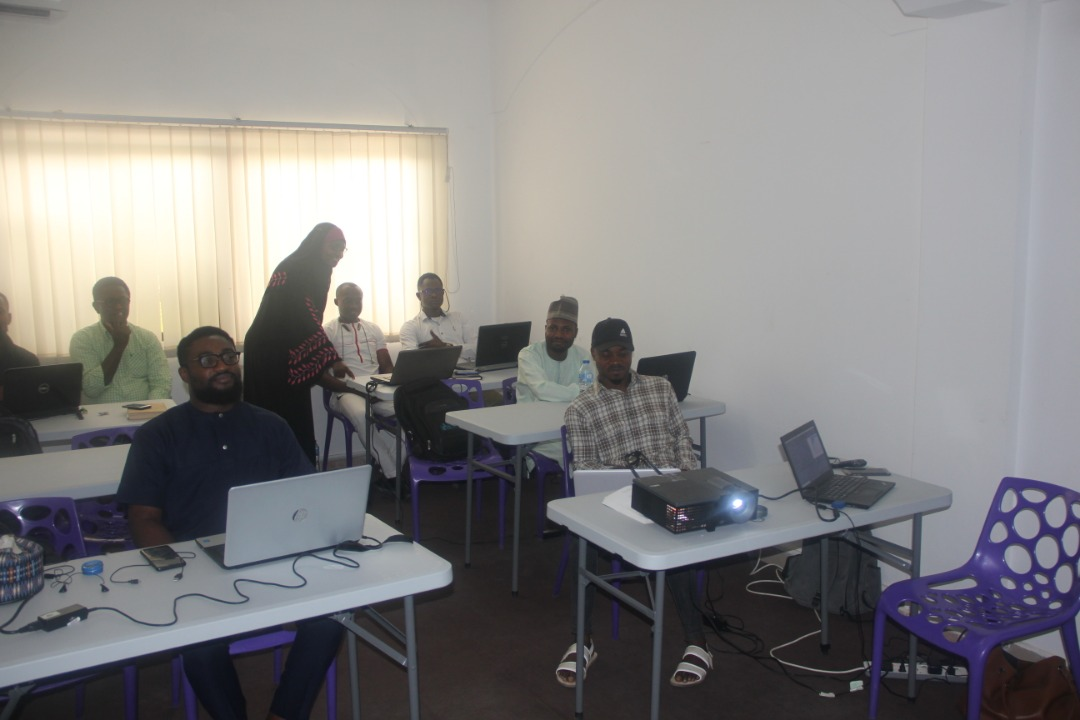
\includegraphics[width=5.19792in,height=5.97917in]{images/trainings/pics2.jpeg}

\begin{center}\rule{0.5\linewidth}{0.5pt}\end{center}

\hypertarget{our-classes---virtual}{%
\subsection{Our Classes - Virtual}\label{our-classes---virtual}}

{1} 2 {3 4 5 6}

\begin{itemize}
\tightlist
\item
  Zoom meetings
\item
  Shared document management
\item
  Recorded classes
\item
  Email/Chat messenger
\item
  Weekly/Weekend Online classes
\end{itemize}

\hypertarget{our-curriculum}{%
\subsection{Our Curriculum}\label{our-curriculum}}

{1} 2 {3 4 5 6}

\begin{itemize}
\tightlist
\item
  Skill-tailored curriculum
\item
  Dedicated and supportive Instructors
\item
  Flexible schedule
\item
  Virtual classes
\item
  Portfolio-ready projects
\end{itemize}

\hypertarget{our-instructors}{%
\subsection{Our Instructors}\label{our-instructors}}

{1} 2 {3 4 5 6}

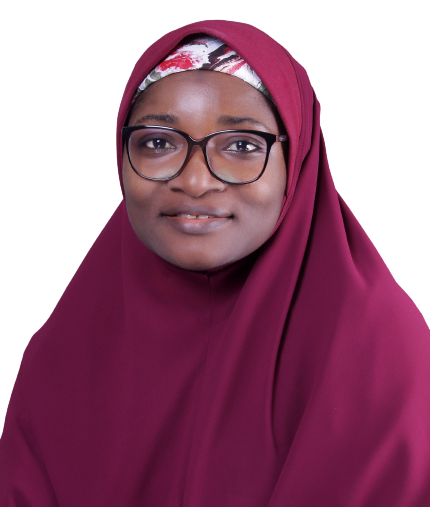
\includegraphics[width=5.19792in,height=5.97917in]{images/profile-pix.png}

Bilikisu Wunmi Olatunji

MSc (Information Technology)

Data Scientist/RShiny Developer

Certified RStudio Instructor, {\textbf{Tidyverse+RShiny}}

Certified {\textbf{Scrum Master/Product Owner/Agile Coach}}

\hypertarget{our-instructors-1}{%
\subsection{Our Instructors}\label{our-instructors-1}}

{1} 2 {3 4 5 6}

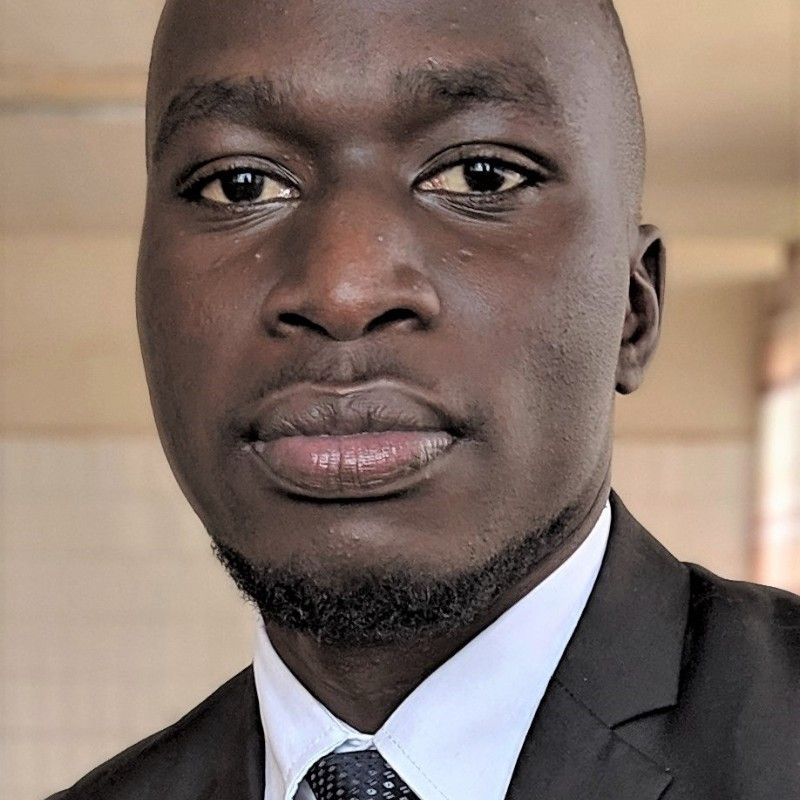
\includegraphics[width=5.19792in,height=5.97917in]{images/robinson.jpg}

Amanyiraho Robinson, Uganda

BSc (Statistics)

Data Scientist/RShiny Developer

Certified RStudio Instructor, {\textbf{Tidyverse}}

\hypertarget{our-instructors-2}{%
\subsection{Our Instructors}\label{our-instructors-2}}

{1} 2 {3 4 5 6}

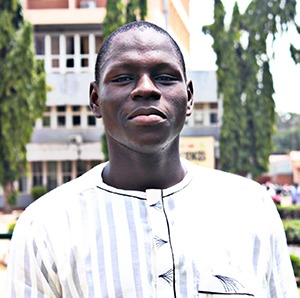
\includegraphics[width=5.19792in,height=5.97917in]{images/ridwan.jpeg}

Adejumo Ridwan Suleiman

BSc (Statistics)

Data Scientist/RShiny Developer

Udemy Instructor

\hypertarget{our-instructors-3}{%
\subsection{Our Instructors}\label{our-instructors-3}}

{1} 2 {3 4 5 6}

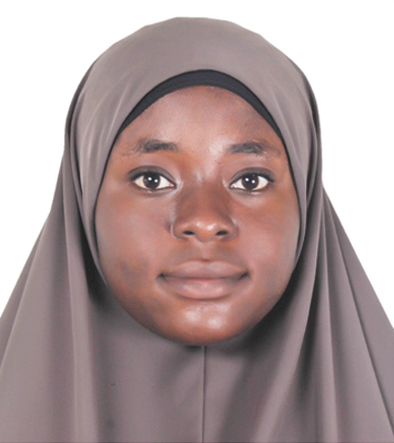
\includegraphics[width=5.19792in,height=5.97917in]{images/faheedah.jpg}

Faheedah Bukola Bello

BSc(Statistics)

Data Scientist/RShiny Developer

Certified Scrum Master

\hypertarget{time-for-todays-workshop}{%
\section{Time for today's Workshop}\label{time-for-todays-workshop}}

{1 2} 3 {4 5 6}

\begin{center}\rule{0.5\linewidth}{0.5pt}\end{center}

\hypertarget{qa}{%
\section{Q/A}\label{qa}}

{1 2 3} 4 {5 6}

\begin{center}\rule{0.5\linewidth}{0.5pt}\end{center}

\hypertarget{thank-you}{%
\section{Thank you}\label{thank-you}}

{1 2 3 4} 5 {6}

\begin{center}\rule{0.5\linewidth}{0.5pt}\end{center}



\end{document}
